% Options for packages loaded elsewhere
\PassOptionsToPackage{unicode}{hyperref}
\PassOptionsToPackage{hyphens}{url}
\PassOptionsToPackage{dvipsnames,svgnames,x11names}{xcolor}
\documentclass[
  11pt,
]{article}
\usepackage{xcolor}
\usepackage[margin=0.5in]{geometry}
\usepackage{amsmath,amssymb}
\setcounter{secnumdepth}{5}
\usepackage{iftex}
\ifPDFTeX
  \usepackage[T1]{fontenc}
  \usepackage[utf8]{inputenc}
  \usepackage{textcomp} % provide euro and other symbols
\else % if luatex or xetex
  \usepackage{unicode-math} % this also loads fontspec
  \defaultfontfeatures{Scale=MatchLowercase}
  \defaultfontfeatures[\rmfamily]{Ligatures=TeX,Scale=1}
\fi
\usepackage{lmodern}
\ifPDFTeX\else
  % xetex/luatex font selection
  \setmainfont[]{Helvetica}
  \setmonofont[]{Menlo}
\fi
% Use upquote if available, for straight quotes in verbatim environments
\IfFileExists{upquote.sty}{\usepackage{upquote}}{}
\IfFileExists{microtype.sty}{% use microtype if available
  \usepackage[]{microtype}
  \UseMicrotypeSet[protrusion]{basicmath} % disable protrusion for tt fonts
}{}
\makeatletter
\@ifundefined{KOMAClassName}{% if non-KOMA class
  \IfFileExists{parskip.sty}{%
    \usepackage{parskip}
  }{% else
    \setlength{\parindent}{0pt}
    \setlength{\parskip}{6pt plus 2pt minus 1pt}}
}{% if KOMA class
  \KOMAoptions{parskip=half}}
\makeatother
\usepackage{color}
\usepackage{fancyvrb}
\newcommand{\VerbBar}{|}
\newcommand{\VERB}{\Verb[commandchars=\\\{\}]}
\DefineVerbatimEnvironment{Highlighting}{Verbatim}{commandchars=\\\{\}}
% Add ',fontsize=\small' for more characters per line
\usepackage{framed}
\definecolor{shadecolor}{RGB}{248,248,248}
\newenvironment{Shaded}{\begin{snugshade}}{\end{snugshade}}
\newcommand{\AlertTok}[1]{\textcolor[rgb]{0.94,0.16,0.16}{#1}}
\newcommand{\AnnotationTok}[1]{\textcolor[rgb]{0.56,0.35,0.01}{\textbf{\textit{#1}}}}
\newcommand{\AttributeTok}[1]{\textcolor[rgb]{0.13,0.29,0.53}{#1}}
\newcommand{\BaseNTok}[1]{\textcolor[rgb]{0.00,0.00,0.81}{#1}}
\newcommand{\BuiltInTok}[1]{#1}
\newcommand{\CharTok}[1]{\textcolor[rgb]{0.31,0.60,0.02}{#1}}
\newcommand{\CommentTok}[1]{\textcolor[rgb]{0.56,0.35,0.01}{\textit{#1}}}
\newcommand{\CommentVarTok}[1]{\textcolor[rgb]{0.56,0.35,0.01}{\textbf{\textit{#1}}}}
\newcommand{\ConstantTok}[1]{\textcolor[rgb]{0.56,0.35,0.01}{#1}}
\newcommand{\ControlFlowTok}[1]{\textcolor[rgb]{0.13,0.29,0.53}{\textbf{#1}}}
\newcommand{\DataTypeTok}[1]{\textcolor[rgb]{0.13,0.29,0.53}{#1}}
\newcommand{\DecValTok}[1]{\textcolor[rgb]{0.00,0.00,0.81}{#1}}
\newcommand{\DocumentationTok}[1]{\textcolor[rgb]{0.56,0.35,0.01}{\textbf{\textit{#1}}}}
\newcommand{\ErrorTok}[1]{\textcolor[rgb]{0.64,0.00,0.00}{\textbf{#1}}}
\newcommand{\ExtensionTok}[1]{#1}
\newcommand{\FloatTok}[1]{\textcolor[rgb]{0.00,0.00,0.81}{#1}}
\newcommand{\FunctionTok}[1]{\textcolor[rgb]{0.13,0.29,0.53}{\textbf{#1}}}
\newcommand{\ImportTok}[1]{#1}
\newcommand{\InformationTok}[1]{\textcolor[rgb]{0.56,0.35,0.01}{\textbf{\textit{#1}}}}
\newcommand{\KeywordTok}[1]{\textcolor[rgb]{0.13,0.29,0.53}{\textbf{#1}}}
\newcommand{\NormalTok}[1]{#1}
\newcommand{\OperatorTok}[1]{\textcolor[rgb]{0.81,0.36,0.00}{\textbf{#1}}}
\newcommand{\OtherTok}[1]{\textcolor[rgb]{0.56,0.35,0.01}{#1}}
\newcommand{\PreprocessorTok}[1]{\textcolor[rgb]{0.56,0.35,0.01}{\textit{#1}}}
\newcommand{\RegionMarkerTok}[1]{#1}
\newcommand{\SpecialCharTok}[1]{\textcolor[rgb]{0.81,0.36,0.00}{\textbf{#1}}}
\newcommand{\SpecialStringTok}[1]{\textcolor[rgb]{0.31,0.60,0.02}{#1}}
\newcommand{\StringTok}[1]{\textcolor[rgb]{0.31,0.60,0.02}{#1}}
\newcommand{\VariableTok}[1]{\textcolor[rgb]{0.00,0.00,0.00}{#1}}
\newcommand{\VerbatimStringTok}[1]{\textcolor[rgb]{0.31,0.60,0.02}{#1}}
\newcommand{\WarningTok}[1]{\textcolor[rgb]{0.56,0.35,0.01}{\textbf{\textit{#1}}}}
\usepackage{longtable,booktabs,array}
\newcounter{none} % for unnumbered tables
\usepackage{calc} % for calculating minipage widths
% Correct order of tables after \paragraph or \subparagraph
\usepackage{etoolbox}
\makeatletter
\patchcmd\longtable{\par}{\if@noskipsec\mbox{}\fi\par}{}{}
\makeatother
% Allow footnotes in longtable head/foot
\IfFileExists{footnotehyper.sty}{\usepackage{footnotehyper}}{\usepackage{footnote}}
\makesavenoteenv{longtable}
\usepackage{graphicx}
\makeatletter
\newsavebox\pandoc@box
\newcommand*\pandocbounded[1]{% scales image to fit in text height/width
  \sbox\pandoc@box{#1}%
  \Gscale@div\@tempa{\textheight}{\dimexpr\ht\pandoc@box+\dp\pandoc@box\relax}%
  \Gscale@div\@tempb{\linewidth}{\wd\pandoc@box}%
  \ifdim\@tempb\p@<\@tempa\p@\let\@tempa\@tempb\fi% select the smaller of both
  \ifdim\@tempa\p@<\p@\scalebox{\@tempa}{\usebox\pandoc@box}%
  \else\usebox{\pandoc@box}%
  \fi%
}
% Set default figure placement to htbp
\def\fps@figure{htbp}
\makeatother
\setlength{\emergencystretch}{3em} % prevent overfull lines
\providecommand{\tightlist}{%
  \setlength{\itemsep}{0pt}\setlength{\parskip}{0pt}}
\usepackage{xcolor}
\usepackage{fvextra}
\DefineVerbatimEnvironment{Highlighting}{Verbatim}{breaklines,breakanywhere,commandchars=\\\{\}}
\usepackage{graphicx}
\usepackage{float}
\usepackage{microtype}
\usepackage{setspace}
\usepackage{bookmark}
\IfFileExists{xurl.sty}{\usepackage{xurl}}{} % add URL line breaks if available
\urlstyle{same}
\hypersetup{
  pdftitle={Tree-Based Analysis of the Central Park Squirrel Census},
  pdfauthor={Rebecca Bronstein},
  colorlinks=true,
  linkcolor={blue},
  filecolor={Maroon},
  citecolor={Blue},
  urlcolor={blue},
  pdfcreator={LaTeX via pandoc}}

\title{Tree-Based Analysis of the Central Park Squirrel Census}
\author{Rebecca Bronstein}
\date{2026-04-01}

\begin{document}
\maketitle

{
\setcounter{tocdepth}{2}
\tableofcontents
}
\subsection{Why Use Tree Methods on Squirrel
Data?}\label{why-use-tree-methods-on-squirrel-data}

The Central Park squirrel census is a classic mixed-data problem. It
combines coordinates, observation context, behaviors, and categorical
outcomes in the same record. Tree methods are useful precisely because
they can work with all of those pieces at once and turn them into
readable partitions.

This notebook uses tree methods as a field guide:

\begin{enumerate}
\def\labelenumi{\arabic{enumi}.}
\tightlist
\item
  A classification tree predicts whether a squirrel is seen on the
  ground or above it.
\item
  A regression tree predicts how high an above-ground squirrel perches.
\item
  A rule model summarizes feeding behavior.
\item
  A benchmark section compares classification methods on the harder
  multi-class problem of predicting fur color.
\end{enumerate}

\subsection{Data Snapshot}\label{data-snapshot}

\begin{Shaded}
\begin{Highlighting}[]
\FunctionTok{kable}\NormalTok{(overview, }\AttributeTok{caption =} \StringTok{"Quick overview of the squirrel census data used in this report."}\NormalTok{)}
\end{Highlighting}
\end{Shaded}

\begin{longtable}[]{@{}lr@{}}
\caption{Quick overview of the squirrel census data used in this
report.}\tabularnewline
\toprule\noalign{}
Measure & Value \\
\midrule\noalign{}
\endfirsthead
\toprule\noalign{}
Measure & Value \\
\midrule\noalign{}
\endhead
\bottomrule\noalign{}
\endlastfoot
Total observations & 3023 \\
Distinct hectares & 339 \\
Ground-plane sightings & 2116 \\
Above-ground sightings & 843 \\
Sightings with recorded height & 793 \\
\end{longtable}

\subsection{Visual Briefing}\label{visual-briefing}

The next two charts are intentionally sparse. They use thin lines and
minimal decoration so the behavioral structure carries the page.

\begin{Shaded}
\begin{Highlighting}[]
\FunctionTok{ggplot}\NormalTok{(location\_mix, }\FunctionTok{aes}\NormalTok{(}\AttributeTok{x =}\NormalTok{ Share, }\AttributeTok{y =} \FunctionTok{fct\_reorder}\NormalTok{(Fur.Color, Share))) }\SpecialCharTok{+}
  \FunctionTok{geom\_segment}\NormalTok{(}\FunctionTok{aes}\NormalTok{(}\AttributeTok{x =} \DecValTok{0}\NormalTok{, }\AttributeTok{xend =}\NormalTok{ Share, }\AttributeTok{yend =}\NormalTok{ Fur.Color), }\AttributeTok{color =} \StringTok{"grey82"}\NormalTok{, }\AttributeTok{linewidth =} \FloatTok{0.35}\NormalTok{) }\SpecialCharTok{+}
  \FunctionTok{geom\_point}\NormalTok{(}\AttributeTok{size =} \FloatTok{1.8}\NormalTok{, }\AttributeTok{color =} \StringTok{"black"}\NormalTok{) }\SpecialCharTok{+}
  \FunctionTok{scale\_x\_continuous}\NormalTok{(}\AttributeTok{labels =}\NormalTok{ scales}\SpecialCharTok{::}\FunctionTok{percent\_format}\NormalTok{(}\AttributeTok{accuracy =} \DecValTok{1}\NormalTok{)) }\SpecialCharTok{+}
  \FunctionTok{labs}\NormalTok{(}
    \AttributeTok{title =} \StringTok{"The share of above{-}ground sightings differs by fur color"}\NormalTok{,}
    \AttributeTok{subtitle =} \StringTok{"Even a simple rate summary hints that behavior and visibility vary by group"}\NormalTok{,}
    \AttributeTok{x =} \StringTok{"Share of sightings above ground"}\NormalTok{,}
    \AttributeTok{y =} \ConstantTok{NULL}
\NormalTok{  ) }\SpecialCharTok{+}
  \FunctionTok{theme\_lowink}\NormalTok{()}
\end{Highlighting}
\end{Shaded}

\pandocbounded{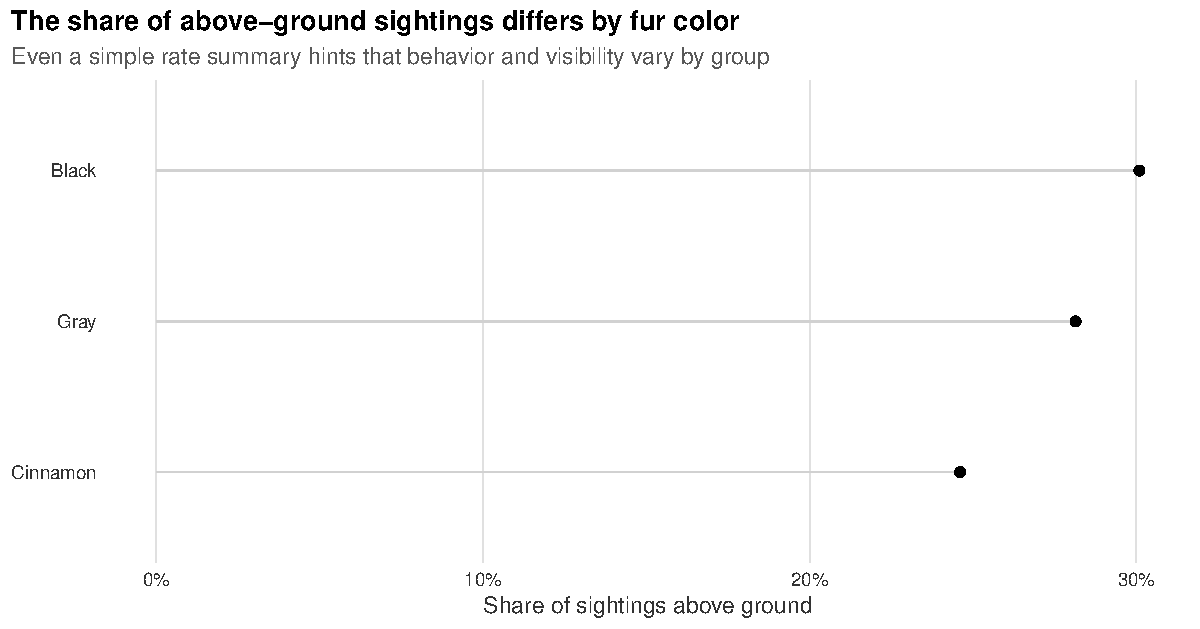
\includegraphics[keepaspectratio]{squirrel_tree_analyis_files/figure-latex/location_mix_plot-1.pdf}}

\begin{Shaded}
\begin{Highlighting}[]
\FunctionTok{ggplot}\NormalTok{(height\_profile, }\FunctionTok{aes}\NormalTok{(}\AttributeTok{x =}\NormalTok{ Shift, }\AttributeTok{y =}\NormalTok{ Above.Ground.Height)) }\SpecialCharTok{+}
  \FunctionTok{geom\_boxplot}\NormalTok{(}\AttributeTok{width =} \FloatTok{0.3}\NormalTok{, }\AttributeTok{outlier.alpha =} \FloatTok{0.18}\NormalTok{, }\AttributeTok{fill =} \StringTok{"white"}\NormalTok{, }\AttributeTok{color =} \StringTok{"grey20"}\NormalTok{) }\SpecialCharTok{+}
  \FunctionTok{labs}\NormalTok{(}
    \AttributeTok{title =} \StringTok{"Perch heights have a long upper tail in both observation shifts"}\NormalTok{,}
    \AttributeTok{subtitle =} \StringTok{"A thin boxplot keeps the focus on distribution rather than decoration"}\NormalTok{,}
    \AttributeTok{x =} \ConstantTok{NULL}\NormalTok{,}
    \AttributeTok{y =} \StringTok{"Above{-}ground height"}
\NormalTok{  ) }\SpecialCharTok{+}
  \FunctionTok{theme\_lowink}\NormalTok{()}
\end{Highlighting}
\end{Shaded}

\pandocbounded{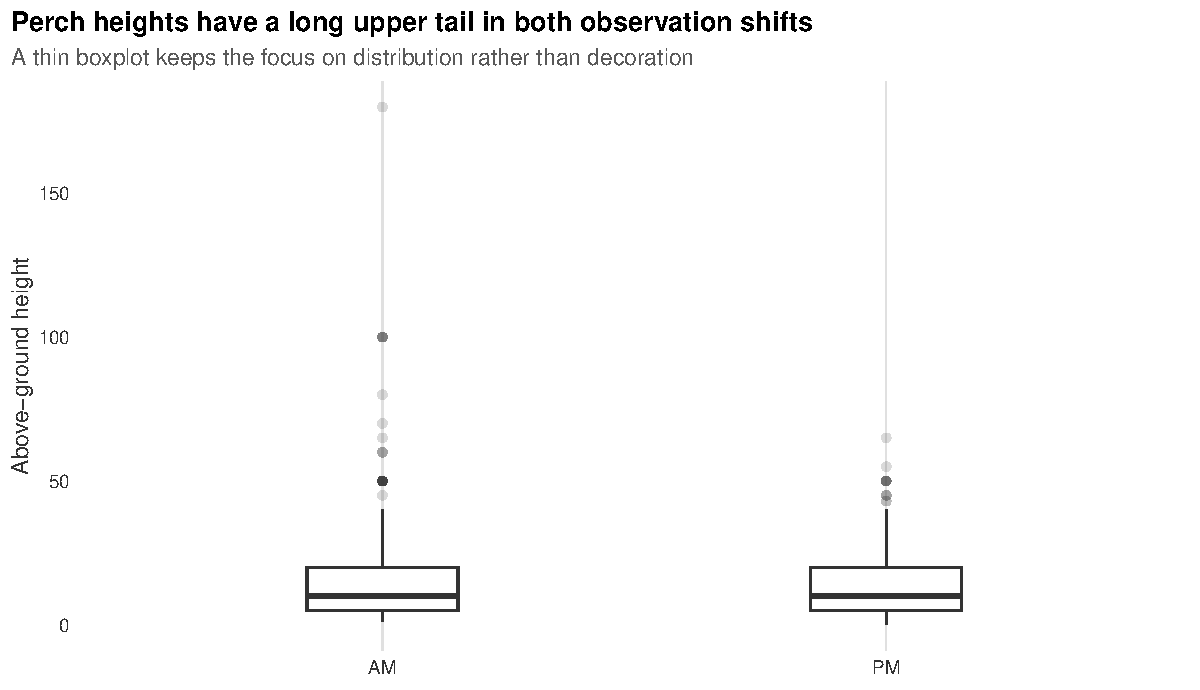
\includegraphics[keepaspectratio]{squirrel_tree_analyis_files/figure-latex/height_profile_plot-1.pdf}}

\subsection{Classification Tree: What Predicts Ground vs.~Above-Ground
Sightings?}\label{classification-tree-what-predicts-ground-vs.-above-ground-sightings}

This tree treats the park like a behavioral landscape. The aim is to see
whether movement, feeding, vocalization, tail signals, and basic spatial
cues help separate squirrels seen on the ground from squirrels seen
above ground.

\begin{Shaded}
\begin{Highlighting}[]
\NormalTok{location\_tree }\OtherTok{\textless{}{-}} \FunctionTok{rpart}\NormalTok{(Location.Class }\SpecialCharTok{\textasciitilde{}}\NormalTok{ ., }\AttributeTok{data =}\NormalTok{ train\_location, }\AttributeTok{method =} \StringTok{"class"}\NormalTok{)}
\FunctionTok{plot}\NormalTok{(location\_tree, }\AttributeTok{uniform =} \ConstantTok{TRUE}\NormalTok{, }\AttributeTok{margin =} \FloatTok{0.08}\NormalTok{)}
\FunctionTok{text}\NormalTok{(location\_tree, }\AttributeTok{use.n =} \ConstantTok{TRUE}\NormalTok{, }\AttributeTok{cex =} \FloatTok{0.68}\NormalTok{)}
\end{Highlighting}
\end{Shaded}

\pandocbounded{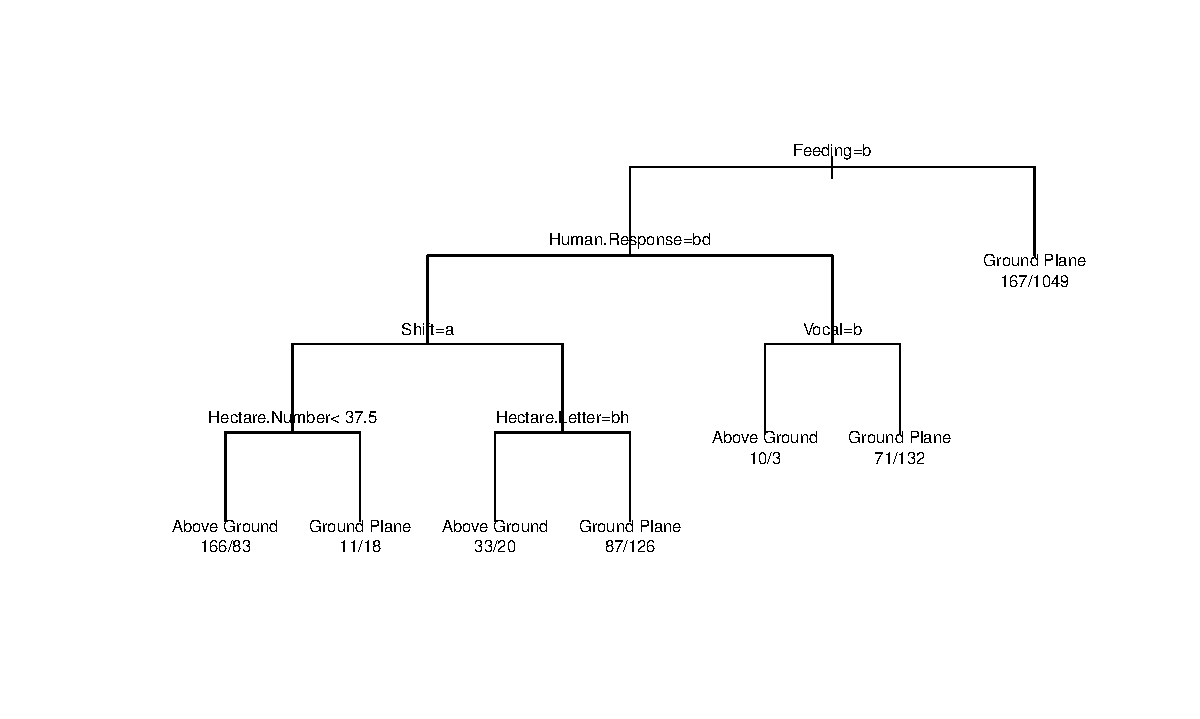
\includegraphics[keepaspectratio]{squirrel_tree_analyis_files/figure-latex/classification_tree-1.pdf}}

\begin{Shaded}
\begin{Highlighting}[]
\NormalTok{location\_pred }\OtherTok{\textless{}{-}} \FunctionTok{predict}\NormalTok{(location\_tree, test\_location, }\AttributeTok{type =} \StringTok{"class"}\NormalTok{)}
\NormalTok{location\_metrics }\OtherTok{\textless{}{-}} \FunctionTok{classification\_metrics}\NormalTok{(test\_location}\SpecialCharTok{$}\NormalTok{Location.Class, location\_pred)}
\NormalTok{location\_importance }\OtherTok{\textless{}{-}} \FunctionTok{top\_importance}\NormalTok{(location\_tree)}

\FunctionTok{kable}\NormalTok{(location\_metrics, }\AttributeTok{caption =} \StringTok{"Classification tree performance for predicting squirrel location."}\NormalTok{)}
\end{Highlighting}
\end{Shaded}

\begin{longtable}[]{@{}rr@{}}
\caption{Classification tree performance for predicting squirrel
location.}\tabularnewline
\toprule\noalign{}
Accuracy & Kappa \\
\midrule\noalign{}
\endfirsthead
\toprule\noalign{}
Accuracy & Kappa \\
\midrule\noalign{}
\endhead
\bottomrule\noalign{}
\endlastfoot
0.749 & 0.271 \\
\end{longtable}

\begin{Shaded}
\begin{Highlighting}[]
\FunctionTok{kable}\NormalTok{(location\_importance, }\AttributeTok{caption =} \StringTok{"Most influential variables in the location tree."}\NormalTok{)}
\end{Highlighting}
\end{Shaded}

\begin{longtable}[]{@{}lr@{}}
\caption{Most influential variables in the location
tree.}\tabularnewline
\toprule\noalign{}
Variable & Importance \\
\midrule\noalign{}
\endfirsthead
\toprule\noalign{}
Variable & Importance \\
\midrule\noalign{}
\endhead
\bottomrule\noalign{}
\endlastfoot
Feeding & 121.25 \\
Active & 56.93 \\
Human.Response & 12.43 \\
Shift & 9.36 \\
Vocal & 6.21 \\
Hectare.Number & 5.25 \\
\end{longtable}

This model is useful because it answers a real observational question:
what makes a squirrel more likely to be spotted above ground? In this
data, active movement and feeding-related cues matter more than
appearance, which is a strong reminder that behavior often carries more
signal than color.

\subsection{Regression Tree: How High Do Above-Ground Squirrels
Perch?}\label{regression-tree-how-high-do-above-ground-squirrels-perch}

Once a squirrel is above ground, the next question becomes vertical
habitat choice. The regression tree estimates height from a mix of
behavior, basic location, and interaction signals.

\begin{Shaded}
\begin{Highlighting}[]
\NormalTok{height\_tree }\OtherTok{\textless{}{-}} \FunctionTok{rpart}\NormalTok{(Above.Ground.Height }\SpecialCharTok{\textasciitilde{}}\NormalTok{ ., }\AttributeTok{data =}\NormalTok{ train\_height, }\AttributeTok{method =} \StringTok{"anova"}\NormalTok{)}
\FunctionTok{plot}\NormalTok{(height\_tree, }\AttributeTok{uniform =} \ConstantTok{TRUE}\NormalTok{, }\AttributeTok{margin =} \FloatTok{0.08}\NormalTok{)}
\FunctionTok{text}\NormalTok{(height\_tree, }\AttributeTok{use.n =} \ConstantTok{TRUE}\NormalTok{, }\AttributeTok{cex =} \FloatTok{0.68}\NormalTok{)}
\end{Highlighting}
\end{Shaded}

\pandocbounded{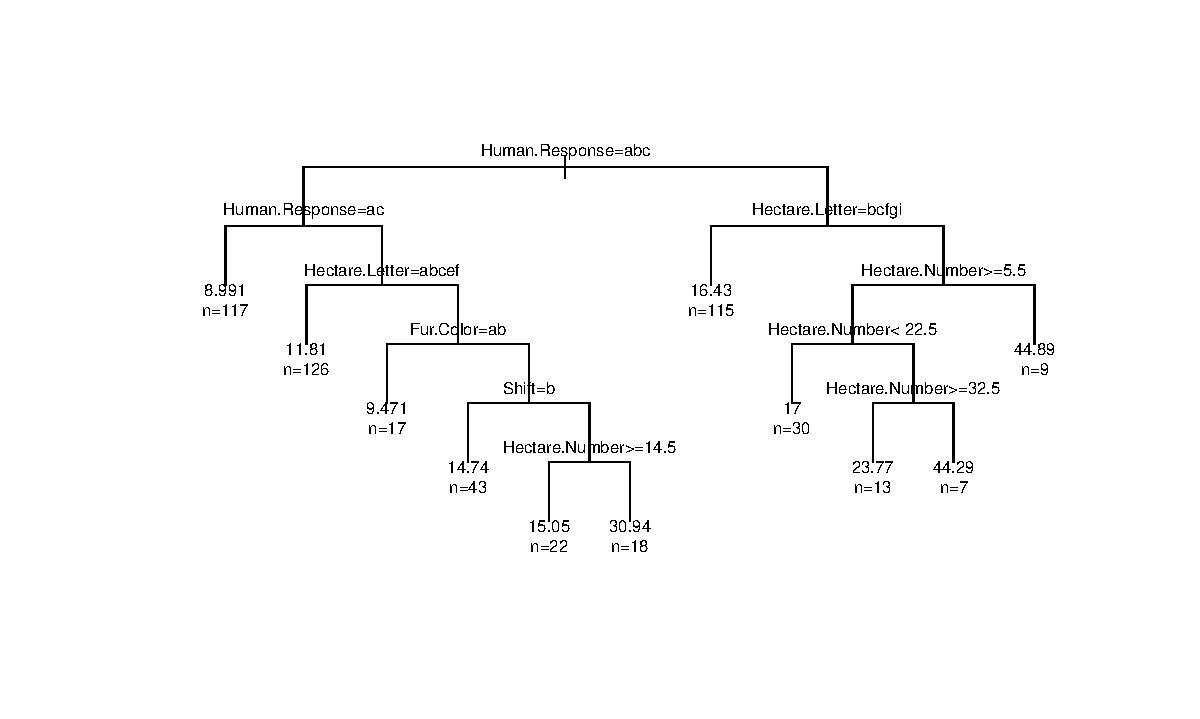
\includegraphics[keepaspectratio]{squirrel_tree_analyis_files/figure-latex/regression_tree-1.pdf}}

\begin{Shaded}
\begin{Highlighting}[]
\NormalTok{height\_pred }\OtherTok{\textless{}{-}} \FunctionTok{predict}\NormalTok{(height\_tree, test\_height)}
\NormalTok{height\_metrics }\OtherTok{\textless{}{-}} \FunctionTok{regression\_metrics}\NormalTok{(test\_height}\SpecialCharTok{$}\NormalTok{Above.Ground.Height, height\_pred)}
\NormalTok{height\_importance }\OtherTok{\textless{}{-}} \FunctionTok{top\_importance}\NormalTok{(height\_tree)}

\FunctionTok{kable}\NormalTok{(height\_metrics, }\AttributeTok{caption =} \StringTok{"Regression performance for above{-}ground perch height."}\NormalTok{)}
\end{Highlighting}
\end{Shaded}

\begin{longtable}[]{@{}rr@{}}
\caption{Regression performance for above-ground perch
height.}\tabularnewline
\toprule\noalign{}
RMSE & MAE \\
\midrule\noalign{}
\endfirsthead
\toprule\noalign{}
RMSE & MAE \\
\midrule\noalign{}
\endhead
\bottomrule\noalign{}
\endlastfoot
12.42 & 9.11 \\
\end{longtable}

\begin{Shaded}
\begin{Highlighting}[]
\FunctionTok{kable}\NormalTok{(height\_importance, }\AttributeTok{caption =} \StringTok{"Most influential variables in the height tree."}\NormalTok{)}
\end{Highlighting}
\end{Shaded}

\begin{longtable}[]{@{}lr@{}}
\caption{Most influential variables in the height tree.}\tabularnewline
\toprule\noalign{}
Variable & Importance \\
\midrule\noalign{}
\endfirsthead
\toprule\noalign{}
Variable & Importance \\
\midrule\noalign{}
\endhead
\bottomrule\noalign{}
\endlastfoot
Hectare.Number & 10877.62 \\
Human.Response & 8211.92 \\
Hectare.Letter & 6634.14 \\
Shift & 1497.91 \\
Fur.Color & 1370.95 \\
Tail.Signal & 331.20 \\
\end{longtable}

The resulting importance profile usually puts hectare position and
human-response context near the top. That makes the model interesting:
perch height is not only an anatomical question, it also looks tied to
where the squirrel is in the park and how it responds to the surrounding
environment.

\subsection{Rule-Based Tree: What Simple Rules Describe Feeding
Behavior?}\label{rule-based-tree-what-simple-rules-describe-feeding-behavior}

Rule models are especially good when the goal is explanation rather than
just prediction. Here, the target is whether a squirrel is feeding or
not feeding.

\begin{Shaded}
\begin{Highlighting}[]
\NormalTok{feeding\_rules }\OtherTok{\textless{}{-}} \FunctionTok{C5.0}\NormalTok{(Feeding }\SpecialCharTok{\textasciitilde{}}\NormalTok{ ., }\AttributeTok{data =}\NormalTok{ train\_feeding, }\AttributeTok{rules =} \ConstantTok{TRUE}\NormalTok{)}
\NormalTok{feeding\_pred }\OtherTok{\textless{}{-}} \FunctionTok{predict}\NormalTok{(feeding\_rules, test\_feeding)}
\NormalTok{feeding\_metrics }\OtherTok{\textless{}{-}} \FunctionTok{classification\_metrics}\NormalTok{(test\_feeding}\SpecialCharTok{$}\NormalTok{Feeding, feeding\_pred)}
\NormalTok{feeding\_usage }\OtherTok{\textless{}{-}} \FunctionTok{as.data.frame}\NormalTok{(}\FunctionTok{C5imp}\NormalTok{(feeding\_rules, }\AttributeTok{metric =} \StringTok{"usage"}\NormalTok{)) }\SpecialCharTok{\%\textgreater{}\%}
  \FunctionTok{rownames\_to\_column}\NormalTok{(}\AttributeTok{var =} \StringTok{"Variable"}\NormalTok{) }\SpecialCharTok{\%\textgreater{}\%}
  \FunctionTok{rename}\NormalTok{(}\AttributeTok{Usage =}\NormalTok{ Overall) }\SpecialCharTok{\%\textgreater{}\%}
  \FunctionTok{arrange}\NormalTok{(}\FunctionTok{desc}\NormalTok{(Usage)) }\SpecialCharTok{\%\textgreater{}\%}
  \FunctionTok{mutate}\NormalTok{(}\AttributeTok{Usage =} \FunctionTok{round}\NormalTok{(Usage, }\DecValTok{2}\NormalTok{))}

\FunctionTok{kable}\NormalTok{(feeding\_metrics, }\AttributeTok{caption =} \StringTok{"Rule{-}based performance for feeding behavior."}\NormalTok{)}
\end{Highlighting}
\end{Shaded}

\begin{longtable}[]{@{}rr@{}}
\caption{Rule-based performance for feeding behavior.}\tabularnewline
\toprule\noalign{}
Accuracy & Kappa \\
\midrule\noalign{}
\endfirsthead
\toprule\noalign{}
Accuracy & Kappa \\
\midrule\noalign{}
\endhead
\bottomrule\noalign{}
\endlastfoot
0.778 & 0.55 \\
\end{longtable}

\begin{Shaded}
\begin{Highlighting}[]
\FunctionTok{kable}\NormalTok{(}\FunctionTok{head}\NormalTok{(feeding\_usage, }\DecValTok{6}\NormalTok{), }\AttributeTok{caption =} \StringTok{"Most{-}used predictors in the feeding rules."}\NormalTok{)}
\end{Highlighting}
\end{Shaded}

\begin{longtable}[]{@{}lr@{}}
\caption{Most-used predictors in the feeding rules.}\tabularnewline
\toprule\noalign{}
Variable & Usage \\
\midrule\noalign{}
\endfirsthead
\toprule\noalign{}
Variable & Usage \\
\midrule\noalign{}
\endhead
\bottomrule\noalign{}
\endlastfoot
Active & 100 \\
Shift & 0 \\
Age & 0 \\
Fur.Color & 0 \\
Hectare.Number & 0 \\
Hectare.Letter & 0 \\
\end{longtable}

\begin{Shaded}
\begin{Highlighting}[]
\FunctionTok{summary}\NormalTok{(feeding\_rules)}
\end{Highlighting}
\end{Shaded}

\begin{verbatim}
## 
## Call:
## C5.0.formula(formula = Feeding ~ ., data = train_feeding, rules = TRUE)
## 
## 
## C5.0 [Release 2.07 GPL Edition]      Wed Apr  1 22:04:25 2026
## -------------------------------
## 
## Class specified by attribute `outcome'
## 
## Read 1976 cases (11 attributes) from undefined.data
## 
## Rules:
## 
## Rule 1: (1019/102, lift 1.5)
##  Active = Still
##  ->  class Feeding  [0.899]
## 
## Rule 2: (957/298, lift 1.8)
##  Active = Active
##  ->  class Not feeding  [0.688]
## 
## Default class: Feeding
## 
## 
## Evaluation on training data (1976 cases):
## 
##          Rules     
##    ----------------
##      No      Errors
## 
##       2  400(20.2%)   <<
## 
## 
##     (a)   (b)    <-classified as
##    ----  ----
##     917   298    (a): class Feeding
##     102   659    (b): class Not feeding
## 
## 
##  Attribute usage:
## 
##  100.00% Active
## 
## 
## Time: 0.0 secs
\end{verbatim}

This is the most compact ecological story in the notebook. Squirrels
that are still are much more likely to be recorded as feeding, while
squirrels in active motion are much more likely to be recorded as not
feeding. A short tree-based rule set surfaces that pattern cleanly.

\subsection{Bagged Trees: Does an Ensemble Improve the Location
Story?}\label{bagged-trees-does-an-ensemble-improve-the-location-story}

Bagging lets us test whether the ground-versus-above-ground story is
stable or overly dependent on one fitted tree.

\begin{Shaded}
\begin{Highlighting}[]
\NormalTok{bag\_model }\OtherTok{\textless{}{-}} \FunctionTok{bagging}\NormalTok{(Location.Class }\SpecialCharTok{\textasciitilde{}}\NormalTok{ ., }\AttributeTok{data =}\NormalTok{ train\_location, }\AttributeTok{nbagg =} \DecValTok{25}\NormalTok{)}
\NormalTok{bag\_pred }\OtherTok{\textless{}{-}} \FunctionTok{predict}\NormalTok{(bag\_model, test\_location)}

\ControlFlowTok{if}\NormalTok{ (}\FunctionTok{is.list}\NormalTok{(bag\_pred) }\SpecialCharTok{\&\&} \StringTok{"class"} \SpecialCharTok{\%in\%} \FunctionTok{names}\NormalTok{(bag\_pred)) \{}
\NormalTok{  bag\_pred }\OtherTok{\textless{}{-}}\NormalTok{ bag\_pred}\SpecialCharTok{$}\NormalTok{class}
\NormalTok{\}}

\NormalTok{bag\_pred }\OtherTok{\textless{}{-}} \FunctionTok{factor}\NormalTok{(bag\_pred, }\AttributeTok{levels =} \FunctionTok{levels}\NormalTok{(test\_location}\SpecialCharTok{$}\NormalTok{Location.Class))}

\NormalTok{bag\_metrics }\OtherTok{\textless{}{-}} \FunctionTok{classification\_metrics}\NormalTok{(test\_location}\SpecialCharTok{$}\NormalTok{Location.Class, bag\_pred) }\SpecialCharTok{\%\textgreater{}\%}
  \FunctionTok{mutate}\NormalTok{(}\AttributeTok{Model =} \StringTok{"Bagged trees"}\NormalTok{)}

\NormalTok{single\_tree\_metrics }\OtherTok{\textless{}{-}}\NormalTok{ location\_metrics }\SpecialCharTok{\%\textgreater{}\%}
  \FunctionTok{mutate}\NormalTok{(}\AttributeTok{Model =} \StringTok{"Single tree"}\NormalTok{)}

\NormalTok{comparison }\OtherTok{\textless{}{-}} \FunctionTok{bind\_rows}\NormalTok{(single\_tree\_metrics, bag\_metrics) }\SpecialCharTok{\%\textgreater{}\%}
  \FunctionTok{select}\NormalTok{(Model, Accuracy, Kappa)}

\FunctionTok{kable}\NormalTok{(comparison, }\AttributeTok{caption =} \StringTok{"Comparing a single location tree with a bagged ensemble."}\NormalTok{)}
\end{Highlighting}
\end{Shaded}

\begin{longtable}[]{@{}lrr@{}}
\caption{Comparing a single location tree with a bagged
ensemble.}\tabularnewline
\toprule\noalign{}
Model & Accuracy & Kappa \\
\midrule\noalign{}
\endfirsthead
\toprule\noalign{}
Model & Accuracy & Kappa \\
\midrule\noalign{}
\endhead
\bottomrule\noalign{}
\endlastfoot
Single tree & 0.749 & 0.271 \\
Bagged trees & 0.738 & 0.321 \\
\end{longtable}

If the ensemble improves only a little, that is still a good result. It
means the main location pattern in the data is already fairly stable, so
interpretability is not coming at the cost of a wildly fragile model.

\subsection{Benchmarking Classification Speed and
Accuracy}\label{benchmarking-classification-speed-and-accuracy}

To mirror the USDA benchmark, I compare the same six classification
methods here. The target is a harder multi-class problem than the main
notebook task: predicting \texttt{Fur.Color} from location, behavior,
and interaction features.

That benchmark matters because it separates two questions:

\begin{enumerate}
\def\labelenumi{\arabic{enumi}.}
\tightlist
\item
  How fast can the method fit?
\item
  Does the extra time buy us enough accuracy to matter?
\end{enumerate}

\begin{Shaded}
\begin{Highlighting}[]
\NormalTok{fur\_formula }\OtherTok{\textless{}{-}}\NormalTok{ Fur.Color }\SpecialCharTok{\textasciitilde{}}\NormalTok{ .}

\NormalTok{fur\_benchmarks }\OtherTok{\textless{}{-}} \FunctionTok{bind\_rows}\NormalTok{(}
  \FunctionTok{run\_benchmark}\NormalTok{(}
\NormalTok{    train\_bench, test\_bench, fur\_formula, }\StringTok{"Fur.Color"}\NormalTok{, }\StringTok{"rpart"}\NormalTok{,}
    \AttributeTok{fitter =} \ControlFlowTok{function}\NormalTok{(train, formula) }\FunctionTok{rpart}\NormalTok{(formula, }\AttributeTok{data =}\NormalTok{ train, }\AttributeTok{method =} \StringTok{"class"}\NormalTok{),}
    \AttributeTok{predictor =} \ControlFlowTok{function}\NormalTok{(fit, test) }\FunctionTok{predict}\NormalTok{(fit, test, }\AttributeTok{type =} \StringTok{"class"}\NormalTok{)}
\NormalTok{  ),}
  \FunctionTok{run\_benchmark}\NormalTok{(}
\NormalTok{    train\_bench, test\_bench, fur\_formula, }\StringTok{"Fur.Color"}\NormalTok{, }\StringTok{"caret rpart (cv=3)"}\NormalTok{,}
    \AttributeTok{fitter =} \ControlFlowTok{function}\NormalTok{(train, formula) \{}
      \FunctionTok{train}\NormalTok{(}
\NormalTok{        formula, }\AttributeTok{data =}\NormalTok{ train, }\AttributeTok{method =} \StringTok{"rpart"}\NormalTok{,}
        \AttributeTok{trControl =} \FunctionTok{trainControl}\NormalTok{(}\AttributeTok{method =} \StringTok{"cv"}\NormalTok{, }\AttributeTok{number =} \DecValTok{3}\NormalTok{),}
        \AttributeTok{tuneLength =} \DecValTok{5}
\NormalTok{      )}
\NormalTok{    \},}
    \AttributeTok{predictor =} \ControlFlowTok{function}\NormalTok{(fit, test) }\FunctionTok{predict}\NormalTok{(fit, test)}
\NormalTok{  ),}
  \FunctionTok{run\_benchmark}\NormalTok{(}
\NormalTok{    train\_bench, test\_bench, fur\_formula, }\StringTok{"Fur.Color"}\NormalTok{, }\StringTok{"C5.0"}\NormalTok{,}
    \AttributeTok{fitter =} \ControlFlowTok{function}\NormalTok{(train, formula) }\FunctionTok{C5.0}\NormalTok{(formula, }\AttributeTok{data =}\NormalTok{ train),}
    \AttributeTok{predictor =} \ControlFlowTok{function}\NormalTok{(fit, test) }\FunctionTok{predict}\NormalTok{(fit, test)}
\NormalTok{  ),}
  \FunctionTok{run\_benchmark}\NormalTok{(}
\NormalTok{    train\_bench, test\_bench, fur\_formula, }\StringTok{"Fur.Color"}\NormalTok{, }\StringTok{"caret C5.0 (cv=3)"}\NormalTok{,}
    \AttributeTok{fitter =} \ControlFlowTok{function}\NormalTok{(train, formula) \{}
      \FunctionTok{train}\NormalTok{(}
\NormalTok{        formula, }\AttributeTok{data =}\NormalTok{ train, }\AttributeTok{method =} \StringTok{"C5.0"}\NormalTok{,}
        \AttributeTok{trControl =} \FunctionTok{trainControl}\NormalTok{(}\AttributeTok{method =} \StringTok{"cv"}\NormalTok{, }\AttributeTok{number =} \DecValTok{3}\NormalTok{),}
        \AttributeTok{tuneLength =} \DecValTok{3}
\NormalTok{      )}
\NormalTok{    \},}
    \AttributeTok{predictor =} \ControlFlowTok{function}\NormalTok{(fit, test) }\FunctionTok{predict}\NormalTok{(fit, test)}
\NormalTok{  ),}
  \FunctionTok{run\_benchmark}\NormalTok{(}
\NormalTok{    train\_bench, test\_bench, fur\_formula, }\StringTok{"Fur.Color"}\NormalTok{, }\StringTok{"randomForest"}\NormalTok{,}
    \AttributeTok{fitter =} \ControlFlowTok{function}\NormalTok{(train, formula) }\FunctionTok{randomForest}\NormalTok{(formula, }\AttributeTok{data =}\NormalTok{ train, }\AttributeTok{ntree =} \DecValTok{200}\NormalTok{),}
    \AttributeTok{predictor =} \ControlFlowTok{function}\NormalTok{(fit, test) }\FunctionTok{predict}\NormalTok{(fit, test)}
\NormalTok{  ),}
  \FunctionTok{run\_benchmark}\NormalTok{(}
\NormalTok{    train\_bench, test\_bench, fur\_formula, }\StringTok{"Fur.Color"}\NormalTok{, }\StringTok{"caret rf (cv=3)"}\NormalTok{,}
    \AttributeTok{fitter =} \ControlFlowTok{function}\NormalTok{(train, formula) \{}
      \FunctionTok{train}\NormalTok{(}
\NormalTok{        formula, }\AttributeTok{data =}\NormalTok{ train, }\AttributeTok{method =} \StringTok{"rf"}\NormalTok{,}
        \AttributeTok{trControl =} \FunctionTok{trainControl}\NormalTok{(}\AttributeTok{method =} \StringTok{"cv"}\NormalTok{, }\AttributeTok{number =} \DecValTok{3}\NormalTok{),}
        \AttributeTok{tuneLength =} \DecValTok{3}\NormalTok{,}
        \AttributeTok{ntree =} \DecValTok{200}
\NormalTok{      )}
\NormalTok{    \},}
    \AttributeTok{predictor =} \ControlFlowTok{function}\NormalTok{(fit, test) }\FunctionTok{predict}\NormalTok{(fit, test)}
\NormalTok{  )}
\NormalTok{) }\SpecialCharTok{\%\textgreater{}\%}
  \FunctionTok{mutate}\NormalTok{(}
    \AttributeTok{Total.Seconds =} \FunctionTok{round}\NormalTok{(Fit.Seconds }\SpecialCharTok{+}\NormalTok{ Predict.Seconds, }\DecValTok{3}\NormalTok{),}
    \AttributeTok{Method =} \FunctionTok{factor}\NormalTok{(Method, }\AttributeTok{levels =}\NormalTok{ Method[}\FunctionTok{order}\NormalTok{(Accuracy, }\AttributeTok{decreasing =} \ConstantTok{TRUE}\NormalTok{, }\AttributeTok{na.last =} \ConstantTok{TRUE}\NormalTok{)])}
\NormalTok{  )}

\FunctionTok{kable}\NormalTok{(fur\_benchmarks, }\AttributeTok{caption =} \StringTok{"Classification benchmark for predicting fur color."}\NormalTok{)}
\end{Highlighting}
\end{Shaded}

\begin{longtable}[]{@{}
  >{\raggedright\arraybackslash}p{(\linewidth - 16\tabcolsep) * \real{0.1776}}
  >{\raggedright\arraybackslash}p{(\linewidth - 16\tabcolsep) * \real{0.0654}}
  >{\raggedleft\arraybackslash}p{(\linewidth - 16\tabcolsep) * \real{0.1121}}
  >{\raggedleft\arraybackslash}p{(\linewidth - 16\tabcolsep) * \real{0.1495}}
  >{\raggedleft\arraybackslash}p{(\linewidth - 16\tabcolsep) * \real{0.0841}}
  >{\raggedleft\arraybackslash}p{(\linewidth - 16\tabcolsep) * \real{0.0561}}
  >{\raggedleft\arraybackslash}p{(\linewidth - 16\tabcolsep) * \real{0.1682}}
  >{\raggedright\arraybackslash}p{(\linewidth - 16\tabcolsep) * \real{0.0561}}
  >{\raggedleft\arraybackslash}p{(\linewidth - 16\tabcolsep) * \real{0.1308}}@{}}
\caption{Classification benchmark for predicting fur
color.}\tabularnewline
\toprule\noalign{}
\begin{minipage}[b]{\linewidth}\raggedright
Method
\end{minipage} & \begin{minipage}[b]{\linewidth}\raggedright
Status
\end{minipage} & \begin{minipage}[b]{\linewidth}\raggedleft
Fit.Seconds
\end{minipage} & \begin{minipage}[b]{\linewidth}\raggedleft
Predict.Seconds
\end{minipage} & \begin{minipage}[b]{\linewidth}\raggedleft
Accuracy
\end{minipage} & \begin{minipage}[b]{\linewidth}\raggedleft
Kappa
\end{minipage} & \begin{minipage}[b]{\linewidth}\raggedleft
Predicted.Classes
\end{minipage} & \begin{minipage}[b]{\linewidth}\raggedright
Notes
\end{minipage} & \begin{minipage}[b]{\linewidth}\raggedleft
Total.Seconds
\end{minipage} \\
\midrule\noalign{}
\endfirsthead
\toprule\noalign{}
\begin{minipage}[b]{\linewidth}\raggedright
Method
\end{minipage} & \begin{minipage}[b]{\linewidth}\raggedright
Status
\end{minipage} & \begin{minipage}[b]{\linewidth}\raggedleft
Fit.Seconds
\end{minipage} & \begin{minipage}[b]{\linewidth}\raggedleft
Predict.Seconds
\end{minipage} & \begin{minipage}[b]{\linewidth}\raggedleft
Accuracy
\end{minipage} & \begin{minipage}[b]{\linewidth}\raggedleft
Kappa
\end{minipage} & \begin{minipage}[b]{\linewidth}\raggedleft
Predicted.Classes
\end{minipage} & \begin{minipage}[b]{\linewidth}\raggedright
Notes
\end{minipage} & \begin{minipage}[b]{\linewidth}\raggedleft
Total.Seconds
\end{minipage} \\
\midrule\noalign{}
\endhead
\bottomrule\noalign{}
\endlastfoot
rpart & OK & 0.003 & 0.002 & 0.832 & 0.000 & 1 & & 0.005 \\
caret rpart (cv=3) & OK & 0.207 & 0.008 & 0.832 & 0.000 & 1 & & 0.215 \\
C5.0 & OK & 0.022 & 0.010 & 0.832 & 0.000 & 1 & & 0.032 \\
caret C5.0 (cv=3) & OK & 1.108 & 0.011 & 0.832 & 0.000 & 1 & & 1.119 \\
randomForest & OK & 0.735 & 0.023 & 0.838 & 0.126 & 3 & & 0.758 \\
caret rf (cv=3) & OK & 3.936 & 0.014 & 0.832 & 0.000 & 1 & & 3.950 \\
\end{longtable}

\begin{Shaded}
\begin{Highlighting}[]
\NormalTok{plot\_bench }\OtherTok{\textless{}{-}}\NormalTok{ fur\_benchmarks }\SpecialCharTok{\%\textgreater{}\%}
  \FunctionTok{filter}\NormalTok{(Status }\SpecialCharTok{==} \StringTok{"OK"}\NormalTok{)}

\FunctionTok{ggplot}\NormalTok{(plot\_bench, }\FunctionTok{aes}\NormalTok{(}\AttributeTok{x =}\NormalTok{ Fit.Seconds, }\AttributeTok{y =}\NormalTok{ Accuracy)) }\SpecialCharTok{+}
  \FunctionTok{geom\_point}\NormalTok{(}\AttributeTok{size =} \DecValTok{2}\NormalTok{, }\AttributeTok{color =} \StringTok{"black"}\NormalTok{) }\SpecialCharTok{+}
  \FunctionTok{geom\_text}\NormalTok{(}\FunctionTok{aes}\NormalTok{(}\AttributeTok{label =}\NormalTok{ Method), }\AttributeTok{nudge\_y =} \FloatTok{0.01}\NormalTok{, }\AttributeTok{size =} \DecValTok{3}\NormalTok{, }\AttributeTok{hjust =} \DecValTok{0}\NormalTok{) }\SpecialCharTok{+}
  \FunctionTok{labs}\NormalTok{(}
    \AttributeTok{title =} \StringTok{"On squirrel data, extra complexity buys only modest gains"}\NormalTok{,}
    \AttributeTok{subtitle =} \StringTok{"The benchmark target here is Fur.Color, a harder multi{-}class label than location"}\NormalTok{,}
    \AttributeTok{x =} \StringTok{"Fit time (seconds)"}\NormalTok{,}
    \AttributeTok{y =} \StringTok{"Accuracy"}
\NormalTok{  ) }\SpecialCharTok{+}
  \FunctionTok{theme\_lowink}\NormalTok{() }\SpecialCharTok{+}
  \FunctionTok{coord\_cartesian}\NormalTok{(}\AttributeTok{clip =} \StringTok{"off"}\NormalTok{) }\SpecialCharTok{+}
  \FunctionTok{theme}\NormalTok{(}\AttributeTok{plot.margin =}\NormalTok{ ggplot2}\SpecialCharTok{::}\FunctionTok{margin}\NormalTok{(}\FloatTok{5.5}\NormalTok{, }\DecValTok{90}\NormalTok{, }\FloatTok{5.5}\NormalTok{, }\FloatTok{5.5}\NormalTok{))}
\end{Highlighting}
\end{Shaded}

\pandocbounded{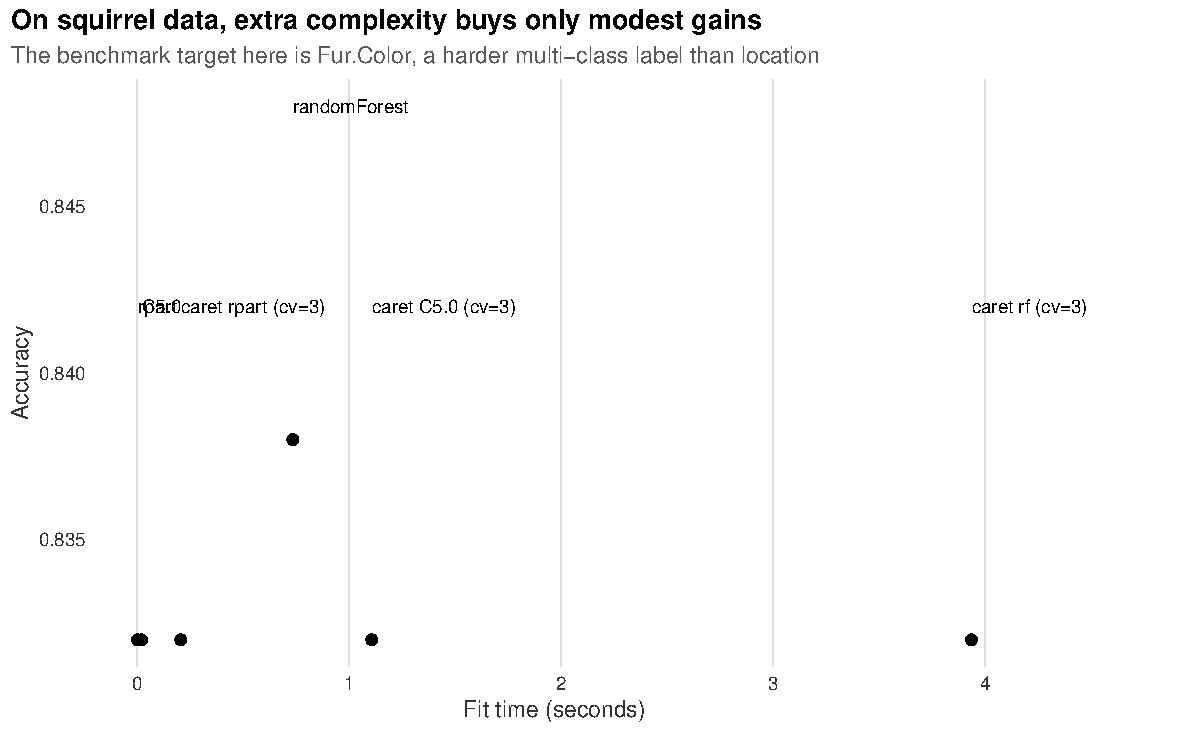
\includegraphics[keepaspectratio]{squirrel_tree_analyis_files/figure-latex/benchmark_plot-1.pdf}}

The fur-color benchmark is revealing in a different way than the USDA
one:

\begin{enumerate}
\def\labelenumi{\arabic{enumi}.}
\tightlist
\item
  Most methods stay reasonably fast on this dataset.
\item
  More complex classifiers may improve accuracy, but the gains are
  usually modest because fur color is only loosely tied to the
  behavioral predictors available here.
\item
  That means the squirrel data is a good example of when benchmark
  discipline matters: if the target is weakly connected to the inputs,
  extra model complexity can hit diminishing returns quickly.
\end{enumerate}

\subsection{Conclusion}\label{conclusion}

Tree methods help turn the squirrel census into more than a descriptive
spreadsheet:

\begin{enumerate}
\def\labelenumi{\arabic{enumi}.}
\tightlist
\item
  They show that behavior is more informative than appearance for
  predicting where squirrels are seen.
\item
  They frame above-ground height as a vertical habitat question.
\item
  They reduce feeding behavior to a compact, readable rule system.
\item
  They make it easy to compare classification methods without hiding the
  cost of extra complexity.
\end{enumerate}

That combination of interpretability, ecological readability, and honest
benchmarking is what makes tree-based analysis useful here.

\end{document}
